\section{Results and discussion}
\label{sec:results}

TODO add figure about evolution of compressibility 

To understand the compressibility of the data produced in a typical
wave-propagation simulation, we ran a simulation as per the setup
described in section TODO, and tried to compress every single timestep
of that simulation and noted the compression ratios achieved at every
timestep. As figure TODO shows, the initial timesteps are much easier
to compress than the later ones. This is not surprising since most
wave simulations start with the field at rest, i.e. filled with zeros.

As the wave reaches more parts of the domain, the field becomes less
compressible until it achieves a stable state when the wave has
reached most of the domain. 

If the simulation had started with the field already oscillating in a
wave, it is likely that the compressibility curve for that simulation
would be flat. 

This tells us that the compressibility of the last timestep of the
solution is representative of the worst-case compressibility and hence
we used the last timestep as our reference for comparison of
compression in the following section. 

The compression ratio achieved per unit time spent during compressing
and decompressing was seen to be highest in the fixed-tolerance mode
albeit with highly unpredictable compression ratios. Figure~\ref{fig:tolerance_cf_plot} shows compression ratios for a variety of
settings for the fixed-tolerance mode. Figure
\ref{fig:decompressed_error} shows the spatial distribution of the
error after compression and decompression, compared to the original
field, using fixed-tolerance mode.
\begin{figure}
\begin{center}
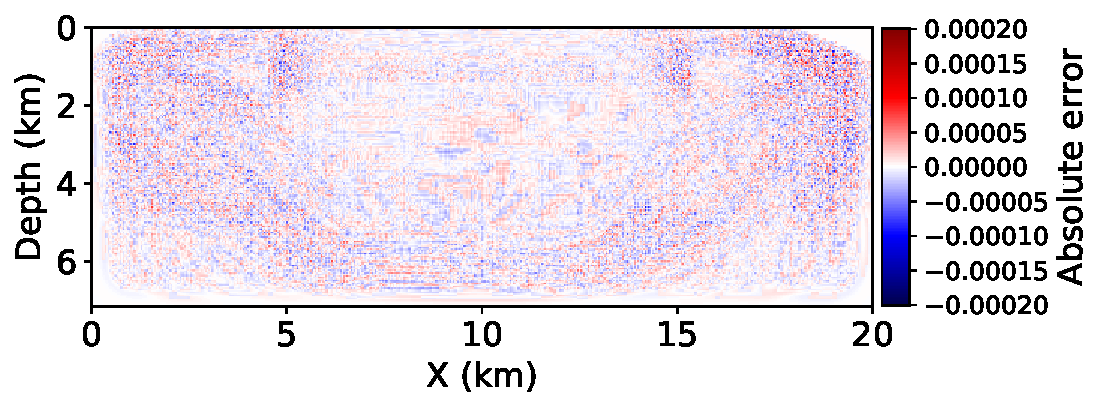
\includegraphics[width=0.8\linewidth]{images/errors.pdf}
\end{center}
\caption{Cross-section of the field that shows errors introduced
  during compression and decompression using the fixed-tolerance
  mode. It is interesting to note that the errors are more or less
  evenly distributed across the domain with only slight variations
  corresponding to the wave amplitude (from the field plot in Figure
  \ref{fig:uncompressed}. A small block-like structure characteristic of
  ZFP can be seen.}
\label{fig:decompressed_error}
\end{figure}


\begin{figure}
\begin{center}
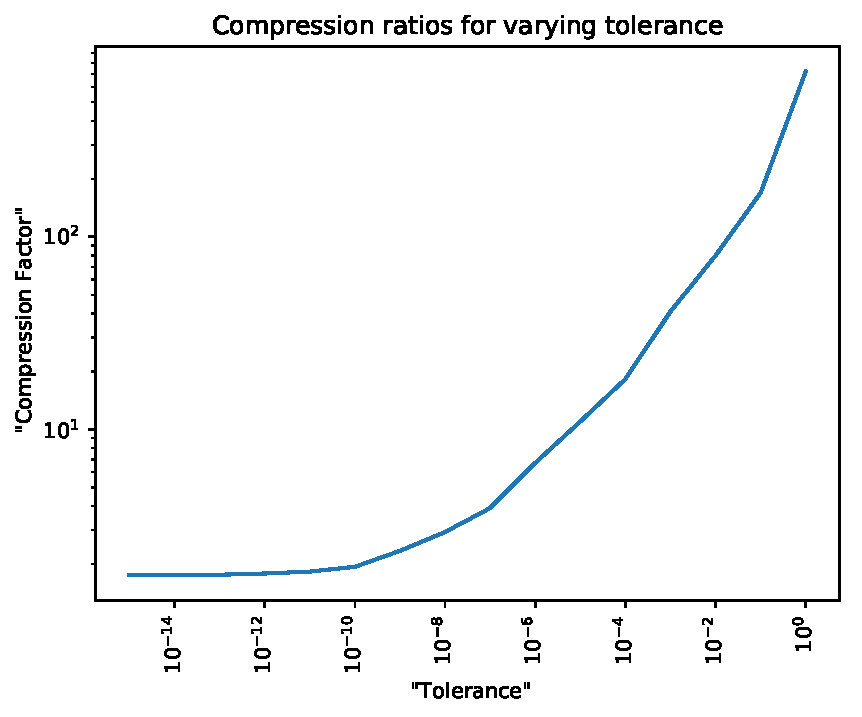
\includegraphics[width=0.9\linewidth]{images/tolerance-cf-richter.pdf}
\end{center}
\caption{Compression ratios achieved on compressing the wavefield. We
  define compression ratio as the ratio between the size of the
  uncompressed data and the compressed data. The dashed line
  represents no compression. The highlighted point corresponds to the
  setting used for the other results here unless otherwise specified.}
\label{fig:tolerance_cf_plot}
\end{figure}

TODO: -Complete forward backward run to calculate gradient and angular
difference with true gradient

We can distinguish three different scenarios, depending on the amount of
available memory.
\begin{enumerate}
\item If the memory is insufficient even with compression to store the entire
trajectory, one can either use checkpointing only, or combine checkpointing with
compression.
\item If the available memory is not sufficient to store the uncompressed
trajectory, but large enough to store the entire compressed trajectory, we study
the two possible strategies: Either use compression only, or use checkpointing
only.
\item If the available system memory is large enough to hold the entire
uncompressed trajectory, neither compression nor checkpointing is necessary.
\end{enumerate}
All three scenarios can be seen in
Figure~\ref{fig:varying_memory}. TODO elaborate on which part of the
figure shows which scenario. 
The second scenario was studied in previous work~\cite{cyr2015towards}, while
the combined method is also applicable to the first scenario, for which previous
work has only used checkpointing without compression.

We can identify a number of factors that make compression more likely to be
beneficial compared to pure checkpointing: A very small system memory size and a
large number of time steps lead to a rapidly increasing recompute factor, and
compression can substantially reduce this recompute factor. This can be seen in
Figures~\ref{fig:varying_memory} and~\ref{fig:varying_nt}.

The extent to which the recompute factor affects the overall runtime also
depends on the cost to compute each individual time step. If the compute cost
per time step is large compared to the compression and decompression cost, then
compression is also likely to be beneficial, as shown in
Figure~\ref{fig:varying_compute}. As the time per time step increases and the
compression cost becomes negligible, we observe that the ratio between the runtime
of the combined method and that of pure checkpointing is only determined by the
difference in recompute factors.

\subsection{Validation of model}
TODO write this section with a plot where theoretical prediction is
shown overlaid with real measurements

Do this for: 
- Acoustic, where compression doesn't pay off
- TTI where compression performs better than recomputation

\begin{figure}
\begin{center}
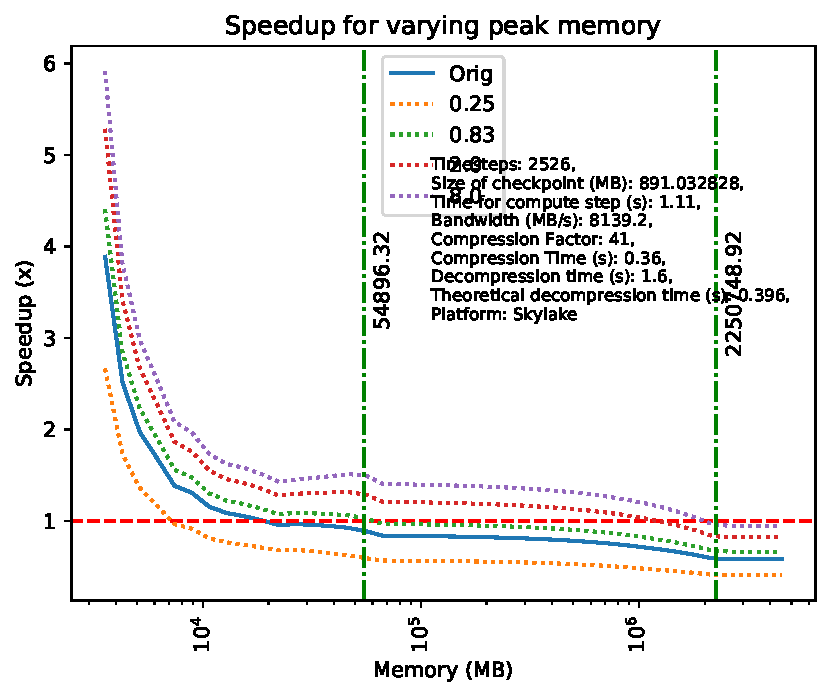
\includegraphics[width=0.9\linewidth]{images/varying-memory.pdf}
\end{center}
\caption{The speedups predicted by the performance model for varying
  memory. The baseline
(1.0) is the performance of a Revolve-only implementation under the
same conditions. The different curves represent kernels with differing
compute times (represented here as a factor of the sum of compression
and decompression times). The first vertical line at $~$ 53GB marks the
spot where the compressed wavefield can completely fit in memory and
Revolve is unnecessary if using compression. The second vertical line
at $~$ 2.2 TB marks the spot where the entire uncompressed wavefield can
fit in memory and neither Revolve nor compression is necessary. The
region to the right is where these optimisations are not necessary or
relevant. The middle region has been the subject of past studies using
compression in adjoint problems. The region to the left is the focus
of this paper.}
\label{fig:varying_memory}
\end{figure}

\begin{figure}
\begin{center}
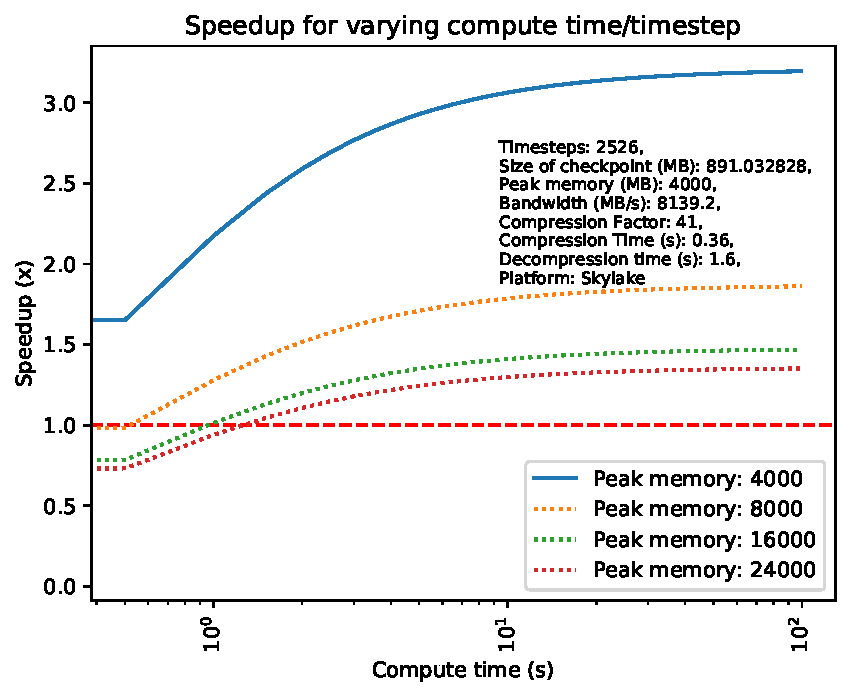
\includegraphics[width=0.9\linewidth]{images/varying-compute.pdf}
\end{center}
\caption{The speedups predicted by the performance model for varying
  compute cost. The baseline
(1.0) is the performance of a Revolve-only implementation under the
same conditions. The benefits of compression drop rapidly if the
computational cost of the kernel that generated the data is much lower
than the cost of compressing the data. For increasing computational
costs, the benefits are bounded.}
\label{fig:varying_compute}
\end{figure}

\begin{figure}
\begin{center}
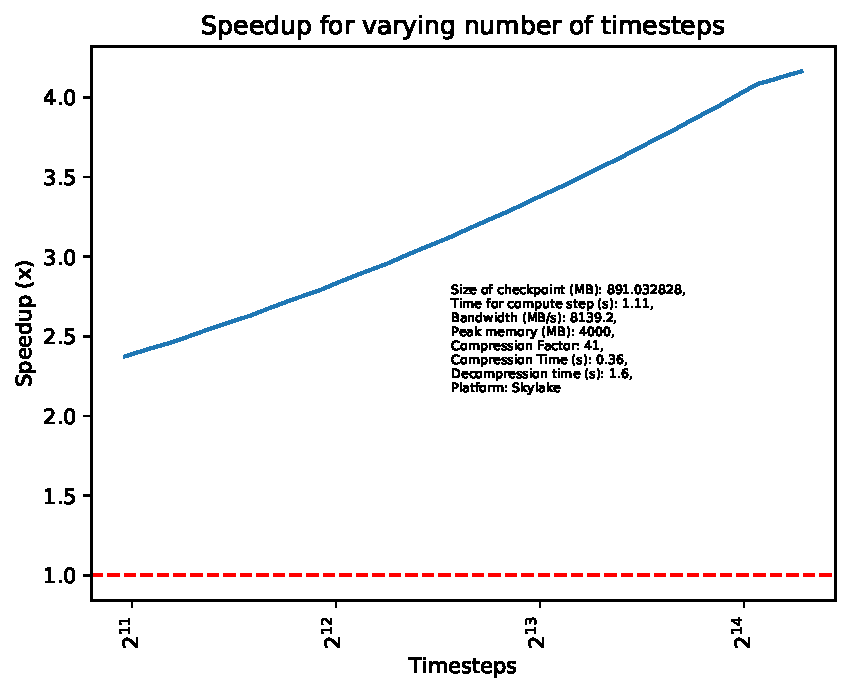
\includegraphics[width=0.9\linewidth]{images/varying-nt.pdf}
\end{center}
\caption{The speedups predicted by the performance model for varying
  number of timesteps to be reversed. The baseline
(1.0) is the performance of a Revolve-only implementation under the
same conditions. It can be seen that compression becomes more
beneficial as the number of timesteps is increased.}
\label{fig:varying_nt}
\end{figure}